\chapter{Стереометрия: плоскости, многогранники и тела вращения}\label{chap:solid-geometry}\markright{Глава 31}

\section{Прямые и плоскости в пространстве}
\begin{definition}\term{Стереометрия} (\emph{solid geometry}) изучает фигуры трёхмерного евклидова пространства. Через три не лежащие на одной прямой точки проходит ровно одна плоскость. Если две точки прямой принадлежат плоскости, вся прямая лежит в ней.\end{definition}
\begin{definition}\term{Скрещивающиеся прямые} (\emph{skew lines}) не лежат в одной плоскости. Они не пересекаются и не являются параллельными.\end{definition}
\begin{definition}\term{Перпендикуляр к плоскости} (\emph{normal line to a plane}) — прямая, перпендикулярная всем проходящим через её основание прямым этой плоскости.\end{definition}
\par\addvspace{5pt}\begin{lrbox}{\CatFlowBox}\begin{minipage}[t]{\linewidth}
\setlength{\parskip}{5pt}\setlength{\columnsep}{4.5mm}\setlength{\intextsep}{0pt}
\begin{wrapfigure}[11]{r}{54mm}
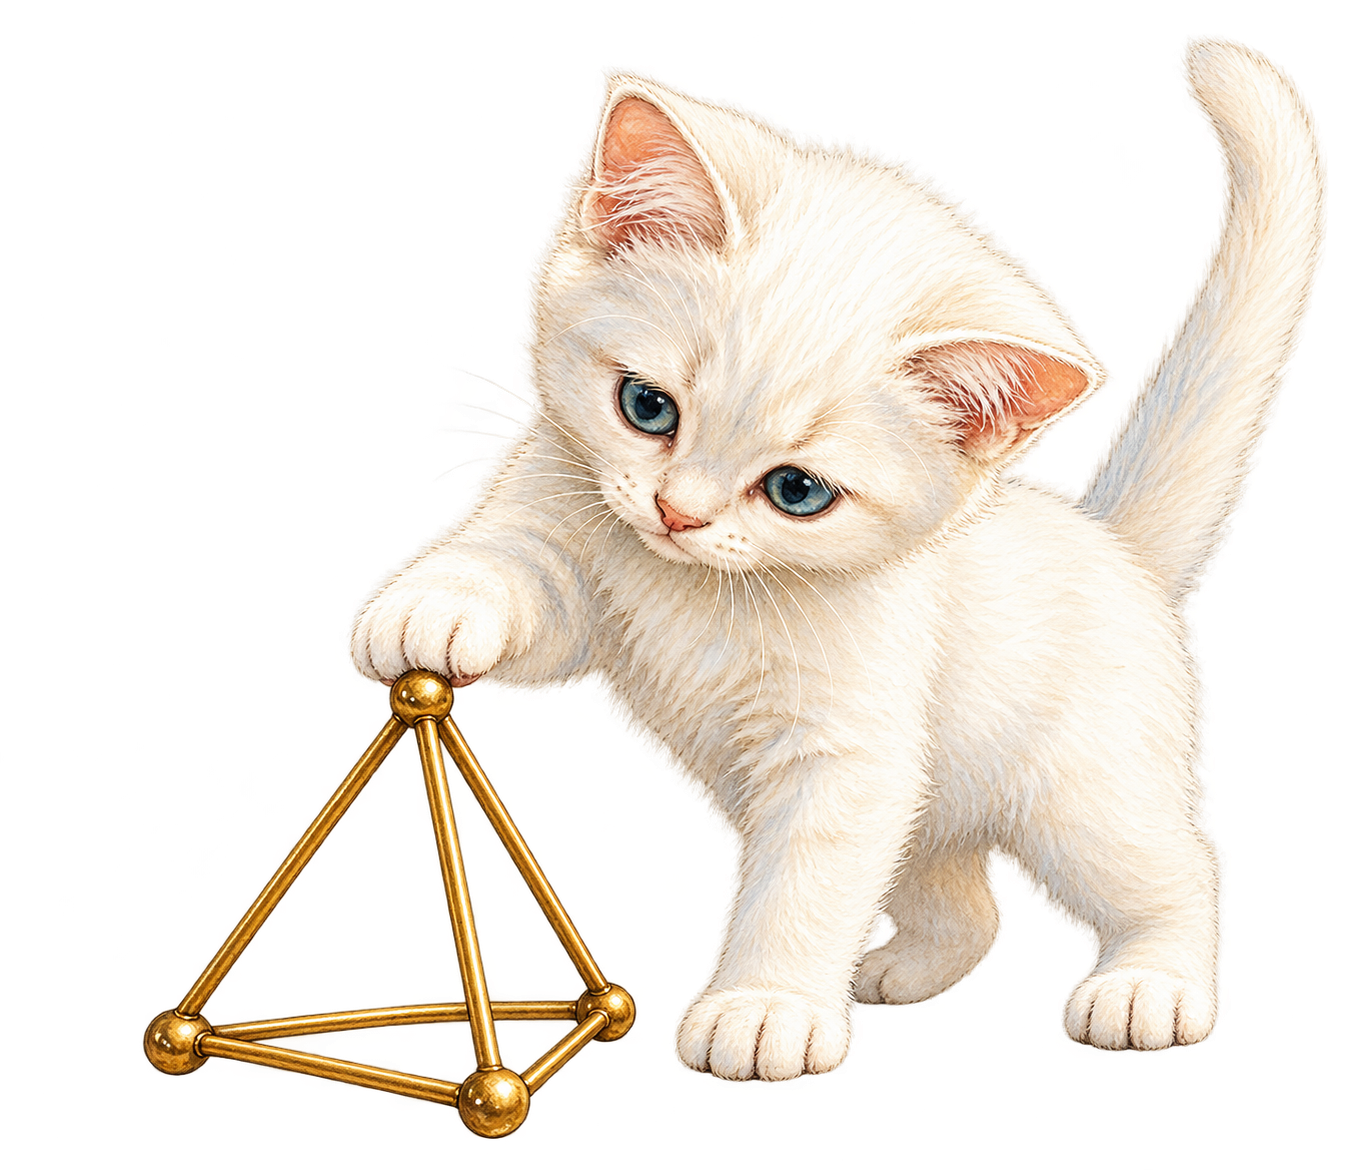
\includegraphics[width=54mm,height=58mm,keepaspectratio]{images/unique/art-142.png}
\end{wrapfigure}
На плоском рисунке пространственные отношения легко перепутать. Проекции скрещивающихся рёбер могут пересекаться, а скрытое ребро может казаться короче видимого. В пространственной задаче сначала устанавливают, какие точки лежат в одной плоскости, затем выбирают сечение, координаты или векторы. Пунктир показывает невидимую часть рисунка, но не является условием о длине.
\par\WFclear\end{minipage}\end{lrbox}%
\ifdim\dimexpr\ht\CatFlowBox+\dp\CatFlowBox\relax<64mm\dp\CatFlowBox=\dimexpr64mm-\ht\CatFlowBox\relax\fi%
\noindent\usebox{\CatFlowBox}\par\addvspace{5pt}
\begin{theorem}[Признак перпендикулярности к плоскости]
Если прямая через \(A\) перпендикулярна двум пересекающимся в \(A\) прямым плоскости, то она перпендикулярна этой плоскости.
\end{theorem}
\begin{proof}Направляющие векторы \(u,v\) этих прямых независимы и порождают все направления плоскости. Если направление \(n\) удовлетворяет \(\langle n,u\rangle=\langle n,v\rangle=0\), то \(\langle n,\alpha u+\beta v\rangle=0\) для любых \(\alpha,\beta\). Это и есть перпендикулярность всем направлениям плоскости.\end{proof}
\begin{definition}\term{Нормальный вектор} (\emph{normal vector}) плоскости — ненулевой вектор, перпендикулярный ей. Плоскость имеет уравнение \(ax+by+cz=d\) с нормалью \(n=(a,b,c)\ne0\).\end{definition}
\begin{theorem}[Расстояние от точки до плоскости]
Для \(P=(x_0,y_0,z_0)\) и плоскости \(ax+by+cz=d\)
\[
\operatorname{dist}(P,\Pi)=
\frac{|ax_0+by_0+cz_0-d|}{\sqrt{a^2+b^2+c^2}}.
\]
\end{theorem}
\begin{proof}Пусть \(Q\) — любая точка плоскости. Проекция \(P-Q\) на единичную нормаль равна \(\frac{\langle n,P-Q\rangle}{\|n\|}\), то есть числу в числителе без модуля, делённому на \(\|n\|\). Перпендикулярная проекция достигает плоскости, а любая наклонная имеет длину не меньше модуля этой компоненты по Пифагору. Получаем наименьшее расстояние.\end{proof}
\section{Углы и векторное произведение}
\begin{definition}\term{Угол между прямыми} (\emph{angle between lines}) выбирают в \([0;\frac\pi2]\). Для ненулевых направлений \(u,v\):
\[
\cos\theta=\frac{|\langle u,v\rangle|}{\|u\|\|v\|}.
\]
\end{definition}
\begin{definition}\term{Угол между прямой и плоскостью} (\emph{line–plane angle}) — угол с её ортогональной проекцией; при нормали \(n\) и направлении \(u\) он задаётся \(\sin\alpha=\frac{|\langle u,n\rangle|}{\|u\|\|n\|}\). Для прямой, перпендикулярной плоскости, принимают \(\alpha=\frac\pi2\).\end{definition}
\begin{definition}\term{Двугранный угол} (\emph{dihedral angle}) образован двумя полуплоскостями с общей граничной прямой; его измеряют углом перпендикулярных к ребру лучей в этих полуплоскостях. При вычислении меньшего угла между двумя плоскостями используют угол между их нормалями с модулем скалярного произведения.\end{definition}
\begin{definition}\term{Векторное произведение} (\emph{cross product}) в правой ортонормированной системе координат имеет вид
\[
u\times v=(u_2v_3-u_3v_2,\ u_3v_1-u_1v_3,\ u_1v_2-u_2v_1).
\]
\end{definition}
\begin{theorem}[Геометрический смысл векторного произведения]
\(u\times v\) перпендикулярен \(u,v\), а его норма равна площади построенного на них параллелограмма:
\[
\|u\times v\|^2=\|u\|^2\|v\|^2-\langle u,v\rangle^2.
\]
При непараллельных \(u,v\) знак направления задаётся правилом правой руки.
\end{theorem}
\begin{proof}Раскрытие скалярных произведений с \(u,v\) даёт ноль. Раскрытие трёх квадратов координат даёт указанное тождество. При угле \(\theta\in[0;\pi]\) его правая часть равна \(\|u\|^2\|v\|^2\sin^2\theta\). Извлечение неотрицательного корня даёт основание, умноженное на высоту. Направление \(e_1\times e_2=e_3\) фиксирует ориентацию; непрерывность сохраняет выбранное правило для непараллельных пар.\end{proof}
\begin{definition}\term{Смешанное произведение} (\emph{scalar triple product}) векторов \(u,v,w\) — число \(\langle u\times v,w\rangle\), равное определителю матрицы с этими столбцами. Для матрицы третьего порядка эта запись означает \[\det[u\ v\ w]=(u_2v_3-u_3v_2)w_1+(u_3v_1-u_1v_3)w_2+(u_1v_2-u_2v_1)w_3.\] Его модуль — объём параллелепипеда: площадь основания умножается на модуль высоты.\end{definition}
\par\addvspace{5pt}\begin{lrbox}{\CatFlowBox}\begin{minipage}[t]{\linewidth}
\setlength{\parskip}{5pt}\setlength{\columnsep}{4.5mm}\setlength{\intextsep}{0pt}
\begin{wrapfigure}[9]{l}{54mm}
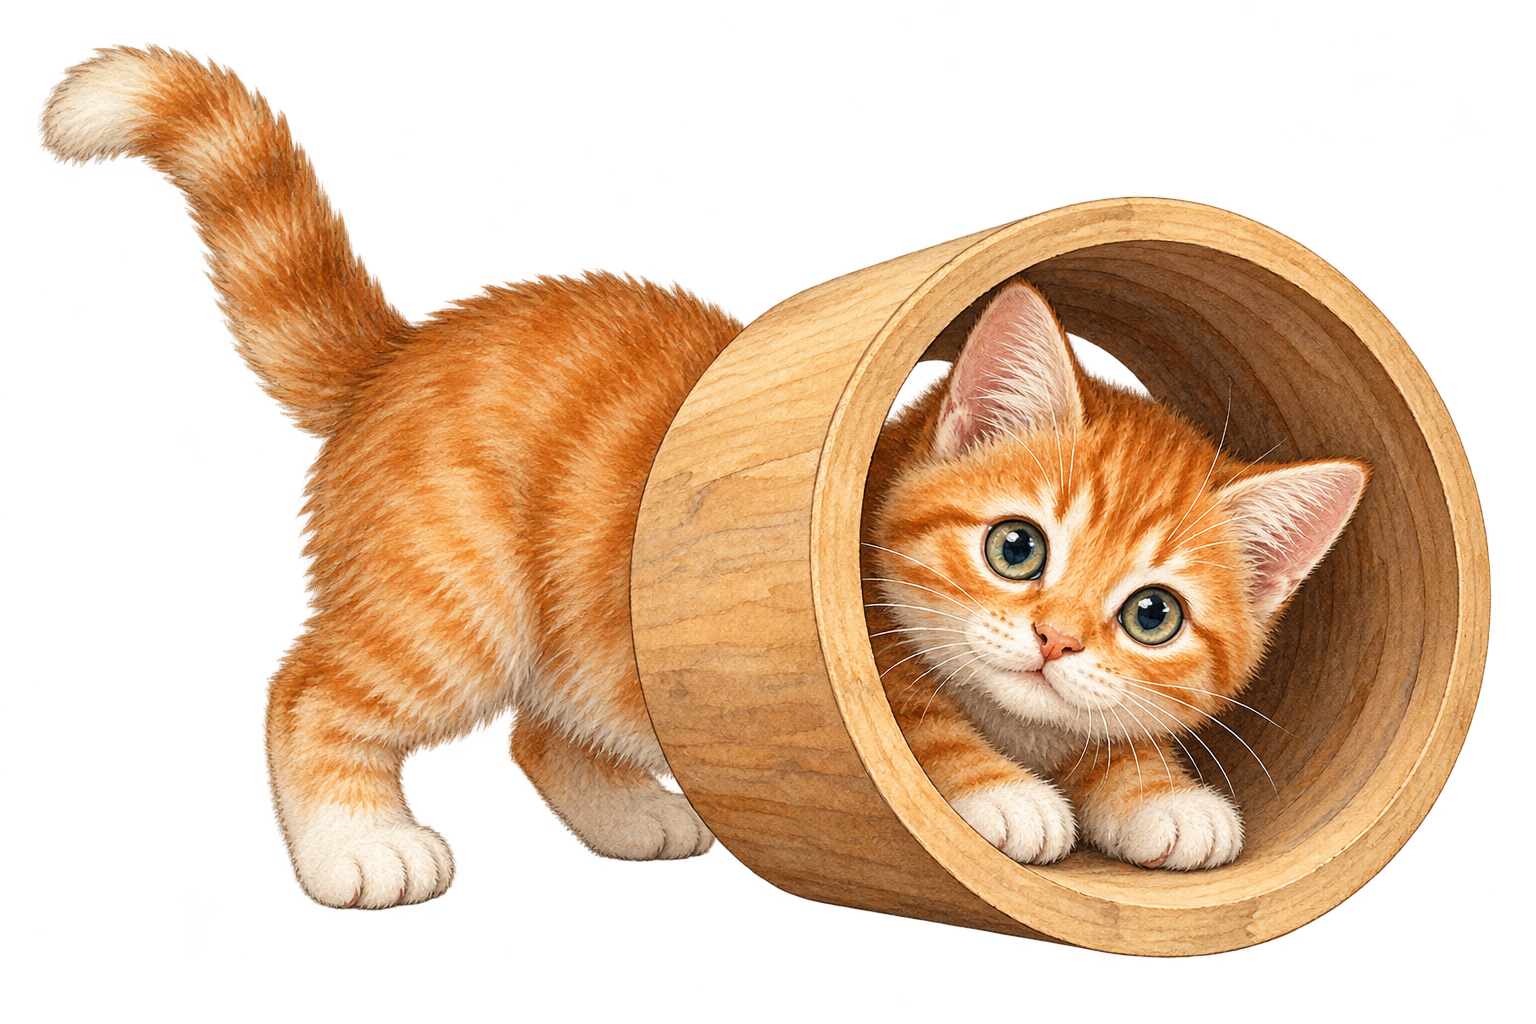
\includegraphics[width=54mm,height=58mm,keepaspectratio]{images/unique/art-143.png}
\end{wrapfigure}
Векторное произведение удобно там, где нужен перпендикуляр сразу к двум направлениям. Его длина отвечает за площадь, а знак направления — за ориентацию. При перестановке множителей \(v\times u=-(u\times v)\). Это пригодится для нормали к поверхности: площадь маленького участка и выбранная сторона поверхности кодируются одним вектором.
\par\WFclear\end{minipage}\end{lrbox}%
\ifdim\dimexpr\ht\CatFlowBox+\dp\CatFlowBox\relax<64mm\dp\CatFlowBox=\dimexpr64mm-\ht\CatFlowBox\relax\fi%
\noindent\usebox{\CatFlowBox}\par\addvspace{5pt}
\section{Многогранники и тела вращения}
\begin{definition}\term{Призма} (\emph{prism}) имеет два равных параллельных многоугольных основания и соединяющие их параллелограммные боковые грани. У прямой призмы боковые рёбра перпендикулярны основаниям.\end{definition}
\begin{definition}\term{Пирамида} (\emph{pyramid}) образована многоугольным основанием и вершиной вне его плоскости; боковые грани — треугольники. Высота — расстояние от вершины до плоскости основания.\end{definition}
\begin{definition}\term{Цилиндр} (\emph{cylinder}), рассматриваемый далее, — прямой круговой цилиндр радиуса \(r\) и высоты \(h\).\end{definition}
\begin{definition}\term{Конус} (\emph{cone}), рассматриваемый далее, — прямой круговой конус радиуса основания \(r\), высоты \(h\) и образующей \(l=\sqrt{r^2+h^2}\).\end{definition}
\begin{definition}\term{Сфера} (\emph{sphere}) с центром \(O\) и радиусом \(R>0\) — множество точек \(P\), для которых \(OP=R\). При \(O=(a,b,c)\) её уравнение \((x-a)^2+(y-b)^2+(z-c)^2=R^2\).\end{definition}
\begin{definition}\term{Замкнутый шар} (\emph{closed ball}) с центром \(O\) и радиусом \(R>0\) — множество точек \(P\), для которых \(OP\le R\). Он состоит из сферы и её внутренности. В координатах \((x-a)^2+(y-b)^2+(z-c)^2\le R^2\); при центре в начале координат получаем \(x^2+y^2+z^2\le R^2\).\end{definition}
\begin{theorem}[Объёмы стандартных тел]\label{thm:solid-volumes}
При площади основания \(B\) и высоте \(h\)
\[
\begin{array}{ll}
\text{призма: }V=Bh,&\text{пирамида: }V=\frac13Bh,\\
\text{цилиндр: }V=\pi r^2h,&\text{конус: }V=\frac13\pi r^2h,\\
\text{шар: }V=\frac43\pi R^3.&
\end{array}
\]
\end{theorem}
Вывод этих формул через площади сечений дан в подразделе \ref{sec:solid-volume-integral}. До введения интеграла ими можно пользоваться как геометрическими формулами.
\begin{theorem}[Площади поверхностей]
Для прямого кругового цилиндра \(S_{\text{бок}}=2\pi rh\), \(S_{\text{полн}}=2\pi rh+2\pi r^2\). Для прямого кругового конуса \(S_{\text{бок}}=\pi rl\), \(S_{\text{полн}}=\pi rl+\pi r^2\). Площадь сферы равна \(4\pi R^2\).
\end{theorem}
\begin{proof}Развёртка боковой поверхности цилиндра — прямоугольник со сторонами \(2\pi r,h\). Развёртка конуса — сектор радиуса \(l\) с дугой \(2\pi r\); его площадь \(\frac12l\cdot2\pi r\). Добавление площадей оснований даёт полные площади. Формула сферы выведена отдельно через поверхностный интеграл в подразделе \ref{sec:sphere-area-integral}.\end{proof}
\par\addvspace{5pt}\begin{lrbox}{\CatFlowBox}\begin{minipage}[t]{\linewidth}
\setlength{\parskip}{5pt}\setlength{\columnsep}{4.5mm}\setlength{\intextsep}{0pt}
\begin{wrapfigure}[13]{r}{54mm}
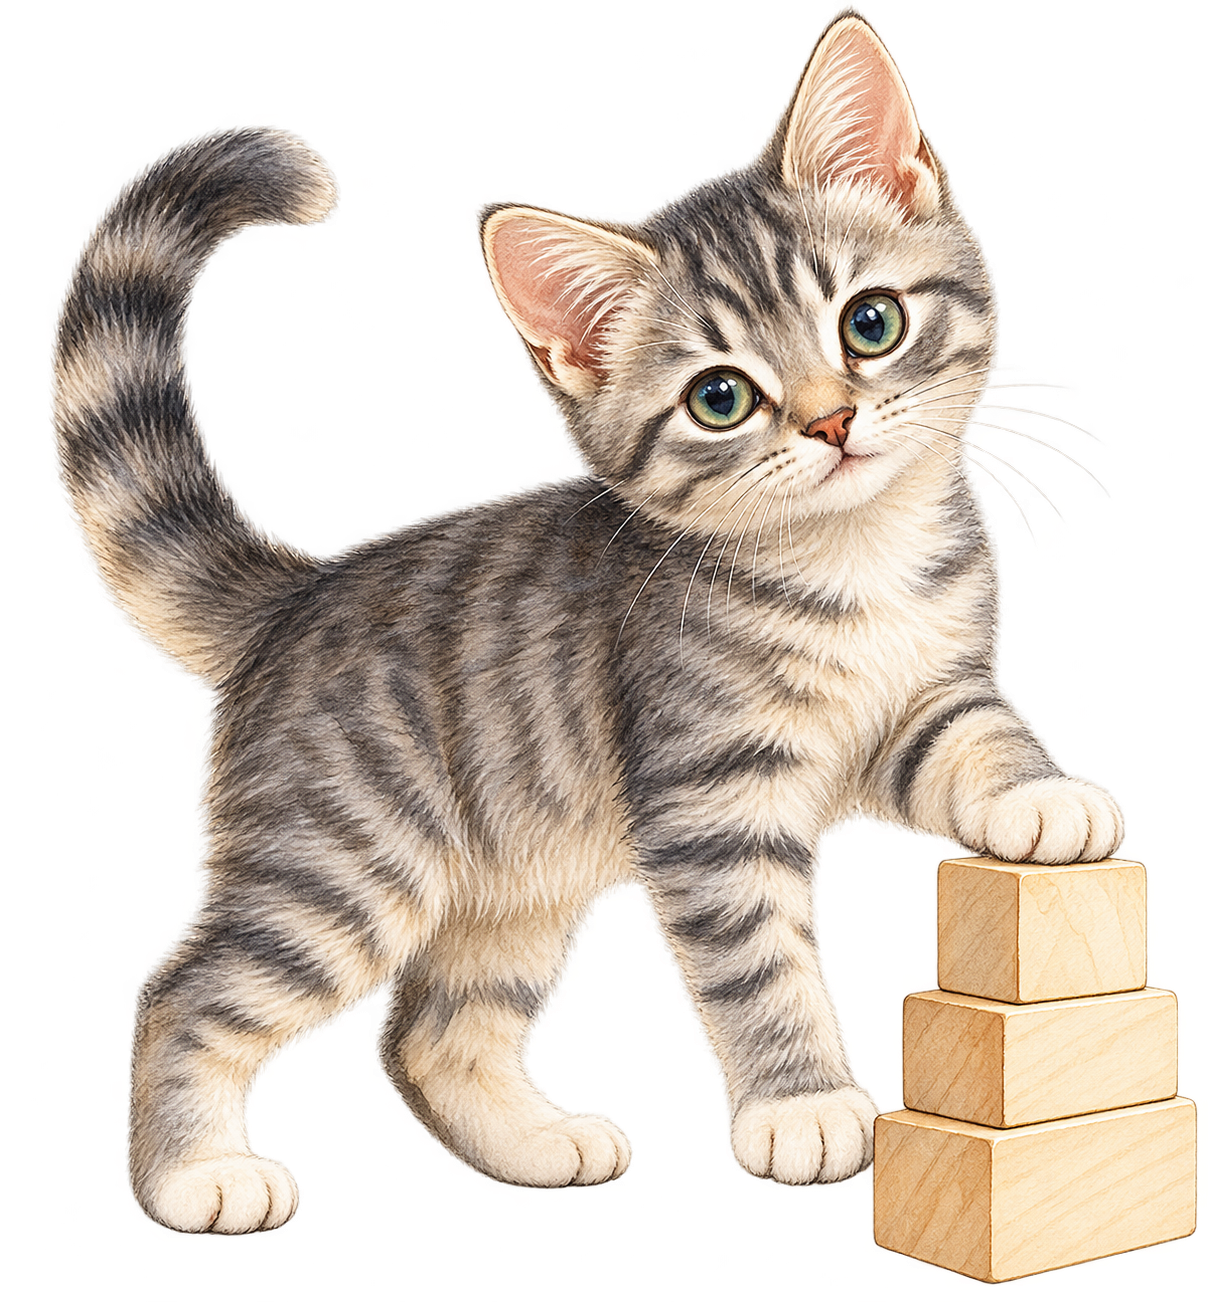
\includegraphics[width=54mm,height=58mm,keepaspectratio]{images/unique/art-144.png}
\end{wrapfigure}
Площадь измеряется в квадратных единицах, объём — в кубических. У подобных тел коэффициент \(k\) увеличивает площади в \(k^2\), объёмы в \(k^3\) раз. Например, модель здания вдвое меньшей высоты при сохранении всех пропорций имеет четверть площади поверхности и одну восьмую объёма. Изменение лишь одной длины не является подобием и такого правила не даёт.
\par\WFclear\end{minipage}\end{lrbox}%
\ifdim\dimexpr\ht\CatFlowBox+\dp\CatFlowBox\relax<64mm\dp\CatFlowBox=\dimexpr64mm-\ht\CatFlowBox\relax\fi%
\noindent\usebox{\CatFlowBox}\par\addvspace{5pt}
\begin{theorem}[Параллельное сечение пирамиды]
Сечение плоскостью, параллельной основанию, на доле \(0<t\le1\) высоты от вершины подобно основанию с коэффициентом \(t\). Его площадь равна \(t^2B\). При \(t=0\) сечение вырождается в вершину и имеет площадь \(0\).
\end{theorem}
\par\addvspace{5pt}\begin{lrbox}{\CatFlowBox}\begin{minipage}[t]{\linewidth}
\setlength{\parskip}{5pt}\setlength{\columnsep}{4.5mm}\setlength{\intextsep}{0pt}
\begin{wrapfigure}[11]{l}{54mm}
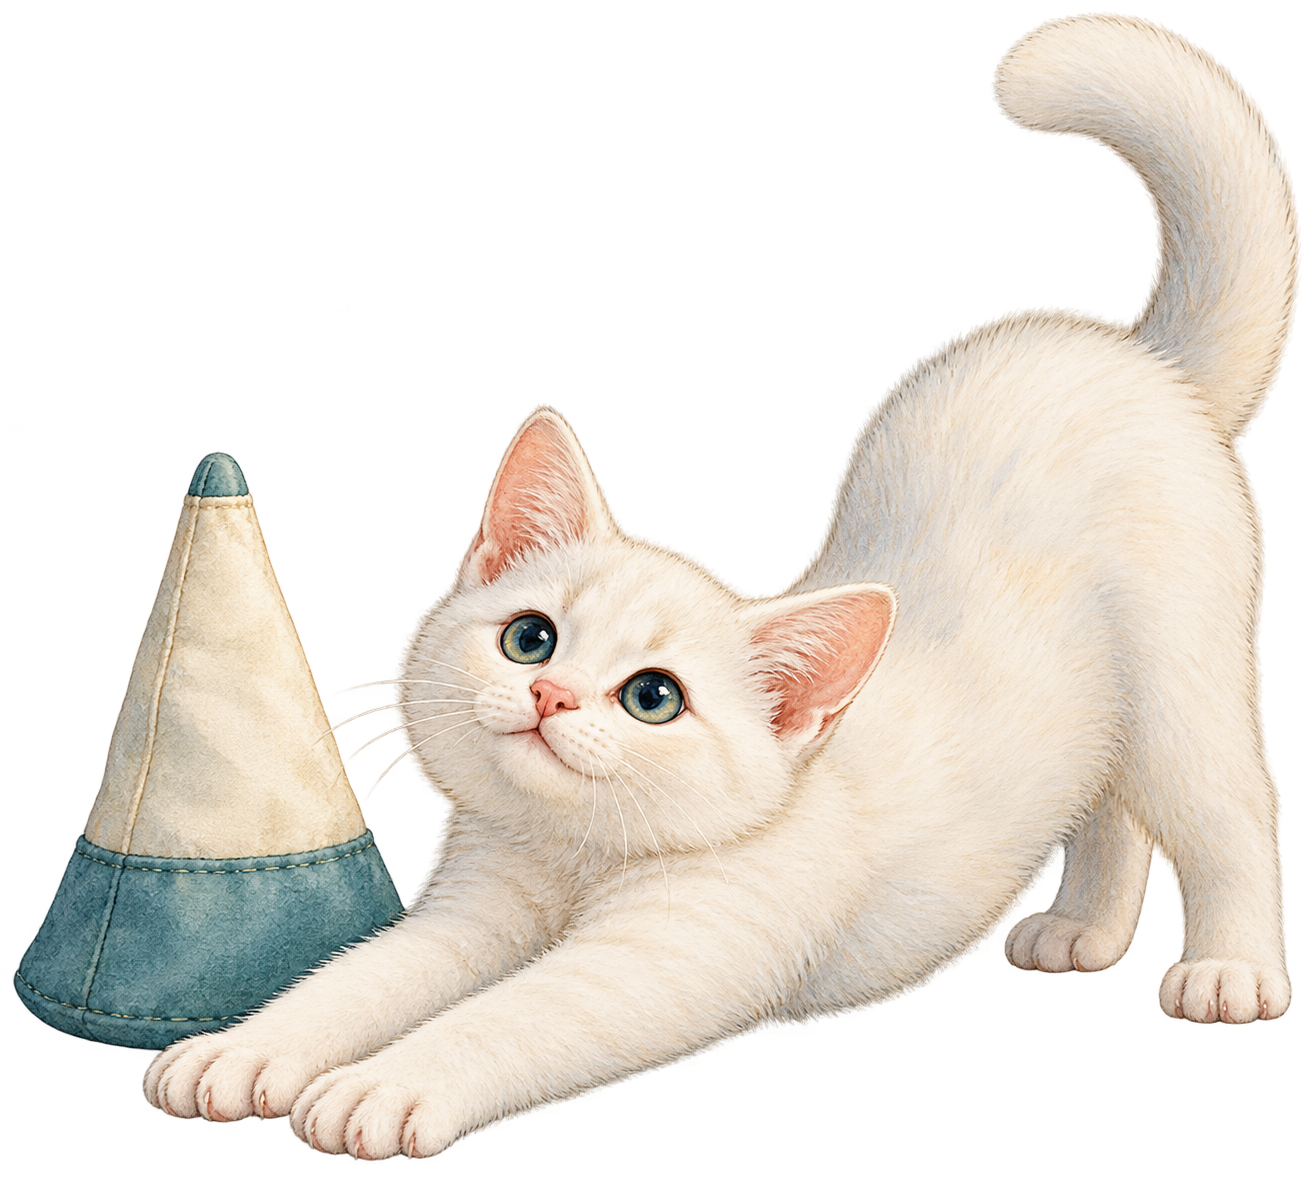
\includegraphics[width=54mm,height=58mm,keepaspectratio]{images/unique/art-145.png}
\end{wrapfigure}
\textit{Доказательство.} На каждом луче из вершины пересечение с параллельной плоскостью делит расстояние до основания в одной доле по подобию плоских треугольников. Поэтому всё сечение получается гомотетией с центром в вершине и коэффициентом \(t\). Площади умножаются на \(t^2\).\hfill\(\blacksquare\)
\par\WFclear\end{minipage}\end{lrbox}%
\ifdim\dimexpr\ht\CatFlowBox+\dp\CatFlowBox\relax<64mm\dp\CatFlowBox=\dimexpr64mm-\ht\CatFlowBox\relax\fi%
\noindent\usebox{\CatFlowBox}\par\addvspace{5pt}


\section{Численные разборы тел вращения}
\begin{example}Цилиндр радиуса \(2\) см и высоты \(5\) см имеет объём \(\pi r^2h=20\pi\) кубических сантиметров. Боковая площадь \(2\pi rh=20\pi\), полная \(2\pi rh+2\pi r^2=28\pi\) квадратных сантиметров. Численные коэффициенты объёма и боковой площади здесь совпали, но это величины разных размерностей.\end{example}
\begin{example}У прямого кругового конуса \(r=3\) см и \(h=4\) см. Образующая \(l=\sqrt{3^2+4^2}=5\) см. Поэтому \(S_{\rm бок}=\pi rl=15\pi\), \(S_{\rm полн}=\pi r(l+r)=24\pi\) квадратных сантиметра, а \(V=\frac13\pi r^2h=12\pi\) кубических сантиметров. Для шара радиуса \(3\) см площадь сферы равна \(36\pi\) квадратных сантиметров, объём шара --- \(36\pi\) кубических сантиметров. Высота конуса входит в объём, образующая --- в боковую площадь; подмена одной другой меняет ответ.\end{example}
\par\noindent\begin{minipage}{\linewidth}\section*{Графики}
\begin{center}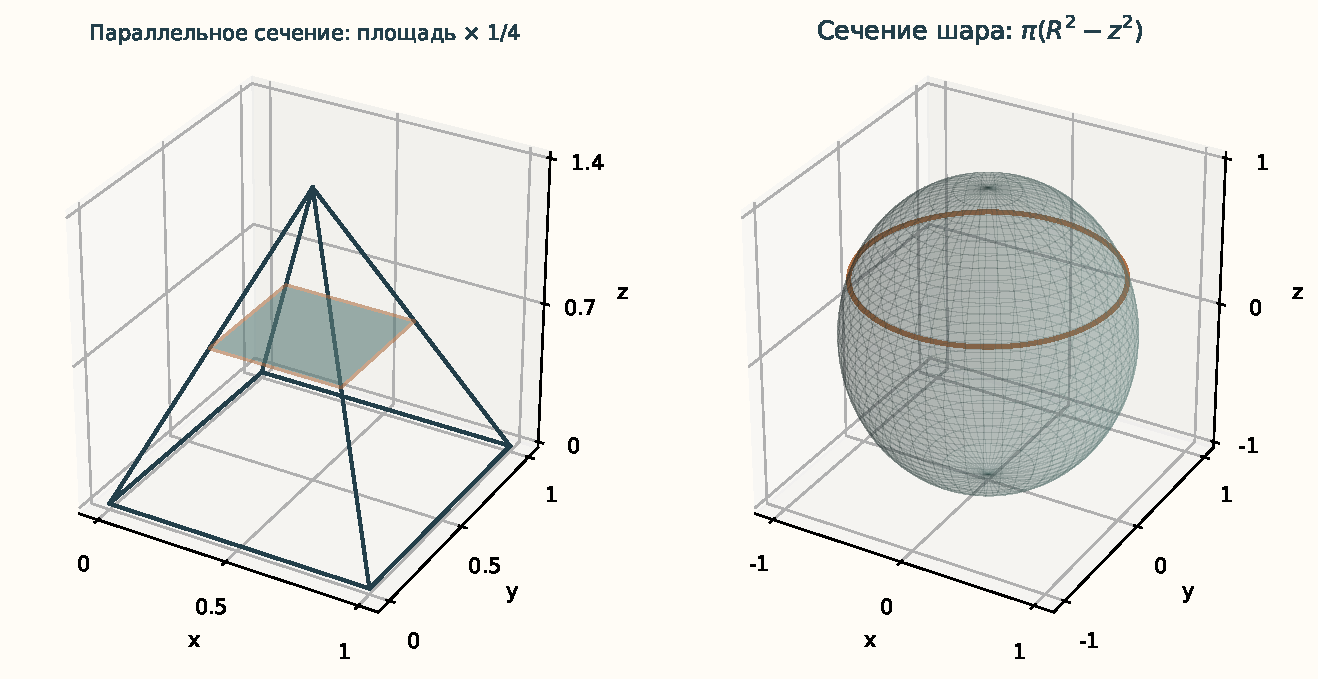
\includegraphics[width=\textwidth,height=.79\textheight,keepaspectratio]{images/atlas-solid-geometry.pdf}\par\small Сечения и объёмы\end{center}\end{minipage}\par
\Needspace{7\baselineskip}\section*{Задачи}
\begingroup\setlength{\parskip}{2pt}
\noindent\begin{minipage}[t]{\linewidth}\textbf{31.1.} У куба ребро \(3\). Найди пространственную диагональ, полную площадь поверхности и объём.\par\end{minipage}\par
\noindent\begin{minipage}[t]{\linewidth}\textbf{31.2.} Площадь основания призмы \(12\), высота \(5\). Найди объём.\par\end{minipage}\par
\noindent\begin{minipage}[t]{\linewidth}\textbf{31.3.} Площадь основания пирамиды \(18\), высота \(4\). Найди объём.\par\end{minipage}\par
\noindent\begin{minipage}[t]{\linewidth}\textbf{31.4.} У цилиндра \(r=2,h=5\). Найди объём, боковую и полную площади поверхности.\par\end{minipage}\par
\noindent\begin{minipage}[t]{\linewidth}\textbf{31.5.} У конуса \(r=3,h=4\). Найди образующую, объём, боковую и полную площади.\par\end{minipage}\par
\par\addvspace{5pt}\begin{lrbox}{\CatFlowBox}\begin{minipage}[t]{\linewidth}
\setlength{\parskip}{5pt}\setlength{\columnsep}{4.5mm}\setlength{\intextsep}{0pt}
\begin{wrapfigure}[11]{r}{54mm}
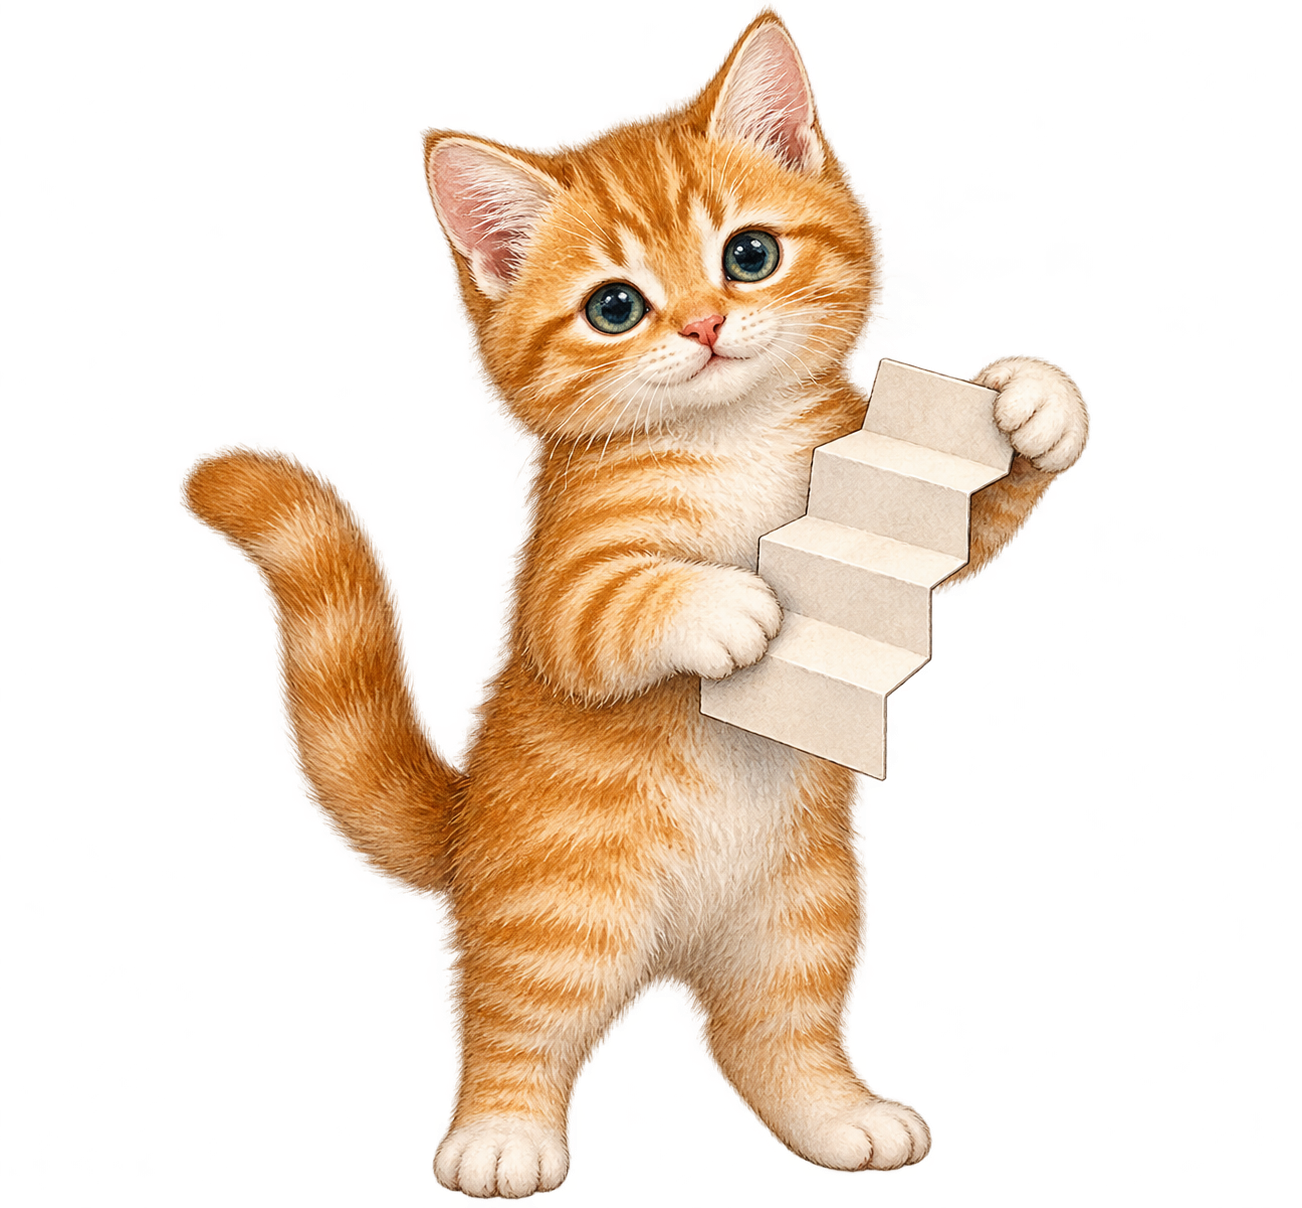
\includegraphics[width=54mm,height=58mm,keepaspectratio]{images/unique/art-146.png}
\end{wrapfigure}
\textbf{31.6.} Найди объём шара и площадь сферы радиуса \(3\).\par

\textbf{31.7.} Объём шара равен \(\dfrac{32\pi}3\). Найди радиус и площадь его границы.\par

\textbf{31.8.} Куб ребра \(4\) пересекают плоскостью, параллельной основанию и проходящей внутри куба. Найди площадь сечения.\par

\textbf{31.9.} Найди расстояние от \(P=(1,2,3)\) до плоскости \(2x-y+2z=9\).\par
\par\WFclear\end{minipage}\end{lrbox}%
\ifdim\dimexpr\ht\CatFlowBox+\dp\CatFlowBox\relax<64mm\dp\CatFlowBox=\dimexpr64mm-\ht\CatFlowBox\relax\fi%
\noindent\usebox{\CatFlowBox}\par\addvspace{5pt}

\noindent\begin{minipage}[t]{\linewidth}\textbf{31.10.} Прямая задана \((x,y,z)=(1,0,0)+t(1,2,2)\). Найди её пересечение с плоскостью \(x+y+z=6\).\par\end{minipage}\par
\noindent\begin{minipage}[t]{\linewidth}\textbf{31.11.} Найди меньший угол между прямыми с направлениями \((1,0,0)\) и \((1,1,0)\).\par\end{minipage}\par
\noindent\begin{minipage}[t]{\linewidth}\textbf{31.12.} Найди угол прямой с направлением \((1,0,1)\) и плоскости \(z=0\).\par\end{minipage}\par
\noindent\begin{minipage}[t]{\linewidth}\textbf{31.13.} Найди меньший угол плоскостей \(x=0\) и \(x+y=0\).\par\end{minipage}\par
\noindent\begin{minipage}[t]{\linewidth}\textbf{31.14.} Для \(u=(1,2,0),v=(0,1,3)\) вычисли \(u\times v\) и площадь параллелограмма.\par\end{minipage}\par
\noindent\begin{minipage}[t]{\linewidth}\textbf{31.15.} Параллелепипед построен на \(u=(1,0,0),v=(0,2,0),w=(1,1,3)\). Найди его объём.\par\end{minipage}\par
\noindent\begin{minipage}[t]{\linewidth}\textbf{31.16.} Найди объём тетраэдра с вершинами \(O,(2,0,0),(0,3,0),(0,0,4)\), где \(O=(0,0,0)\).\par\end{minipage}\par
\noindent\begin{minipage}[t]{\linewidth}\textbf{31.17.} У прямоугольного параллелепипеда рёбра \(3,4,12\). Найди пространственную диагональ.\par\end{minipage}\par
\noindent\begin{minipage}[t]{\linewidth}\textbf{31.18.} Прямоугольный бассейн имеет размеры \(6\) м, \(4\) м и глубину \(1{,}5\) м. Каков объём при заполнении до краёв?\par\end{minipage}\par
\noindent\begin{minipage}[t]{\linewidth}\textbf{31.19.} Нужно покрыть краской закрытую цилиндрическую модель с \(r=1,h=3\). Найди площадь покрытия, включая оба основания.\par\end{minipage}\par
\noindent\begin{minipage}[t]{\linewidth}\textbf{31.20.} Конус пересечён плоскостью, параллельной основанию, на половине высоты от вершины. Во сколько раз меньше площадь сечения и объём малого конуса?\par\end{minipage}\par
\noindent\begin{minipage}[t]{\linewidth}\textbf{31.21.}\starmark{} Докажи, что при подобии с коэффициентом \(k>0\) объём параллелепипеда умножается на \(k^3\).\par\end{minipage}\par
\noindent\begin{minipage}[t]{\linewidth}\textbf{31.22.}\starmark{} Прямые заданы \((t,0,0)\) и \((0,s,2)\), \(t,s\in\mathbb R\). Докажи, что они скрещиваются, и найди расстояние между ними.\par\end{minipage}\par
\noindent\begin{minipage}[t]{\linewidth}\textbf{31.23.}\starmark{} Куб вписан в сферу радиуса \(R\). Вырази его ребро и объём через \(R\).\par\end{minipage}\par
\noindent\begin{minipage}[t]{\linewidth}\textbf{31.24.}\starmark{} У правильного тетраэдра ребро \(a>0\). Найди высоту, площадь поверхности и объём.\par\end{minipage}\par
\noindent\begin{minipage}[t]{\linewidth}\textbf{31.25.} У цилиндра радиус \(3\) см, высота \(7\) см. Найди объём и полную площадь поверхности.\par\end{minipage}\par
\noindent\begin{minipage}[t]{\linewidth}\textbf{31.26.} У прямого кругового конуса радиус \(5\) см и образующая \(13\) см. Найди высоту, объём и полную площадь.\par\end{minipage}\par
\endgroup
